\documentclass{article}
\usepackage[utf8]{inputenc}
\RequirePackage[numbers]{natbib}
\usepackage[intoc,french]{nomencl}
\makenomenclature
\renewcommand{\nomname}{Notations}
\usepackage{etoolbox}
\usepackage{subcaption}
\usepackage{graphicx}
\usepackage{enumitem} 
\usepackage{fancyhdr}
\usepackage[utf8]{inputenc}
\usepackage{amsmath, amssymb, amsthm}
\usepackage{placeins}
\usepackage[top=3cm, bottom=3cm, left=2cm, right=2cm]{geometry}

\title{Spécification d'histogrammes dans le cas de zones constantes}
\author{Pierre Dubreuil, Thomas Eboli}

\begin{document}
\maketitle

\begin{abstract}
Dans ce rapport, nous allons présenter nos résultats au sujet d'application de la spécification d'histogrammes au traitement des images. Nous nous sommes appuyé sur le code fourni par madame Nikolova ainsi que sur le papier de base. La première étape du travail, en amont de tout bout de code a été de comprendre les enjeux soulevés par le papier et d'appréhender la puissance du speed-up de la phase "d'ordering" dans le problème de la spécification d'histogrammes. L'un des principaux problèmes que nous avons cherché à résoudre est l'a présence de "large pixels" dans les images obtenues après spécification. Nos méthodes de résolution reposent sur des considérations probabilistes sur les histogrammes, comme la forme de la distribution de probabilité d'une variable aléatoire $X$ qui est ici l'image.
\end{abstract}

\paragraph*{}
Ce document est organisé comme suit: la partie 1 est dédiée à présenter le problème de "large pixels" et d'en comprendre la source. La partie 2 présente nos premières approches pour résoudre le problème ainsi que que les résultats obtenus. La partie 3 s'intéressera à la méthode la plus satisfaisante de notre point de vue. IL s'agit de combiner la détexttion de pics dans l'histogramme avec des techniques dites "TMR".

\section{Présentation du problème de "large pixels"}
\paragraph*{}
Lors de l'application de l'algorithme donné, on s'aperçoit que les images font apparaître des détails que l'on ne veut pas. La figure \ref{fig:p1_brasil} illustre à merveille ce phénomène qui découle de la mauvaise quantification de la palette de couleurs dans la nouvelle configurations de bits de couleurs. En effet les figures \ref{fig:im_x} et \ref{fig:im_xx} montrent que la spécification d'histogramme, lorsque l'histogramme cible est très différent de l'original, déplace des pixels d'un certain niveau de couleur vers des régions où il n'y avait pas de pixels pour colorer avec cette teinte. Le résultat est visible sur ces figures; le contraste est beaucoup plus riche et la photographie du port de Malte est moins terne mais on fait apparaître dans le ciel des blocs de pixels blancs. Ces pixels sont le résultat d'une volonté de rendre plus contrastée cette zone de l'image mais l'image originale ne possédant qu'une zone quasi constante de couleurs, la nouvelle allocation arrive à rendre le dégradé souhaité que par de gros tas de pixels, les "large pixels". Il faut donc arriver à trouver une technique permettant de gommer ces détails liés à des zones planes dans les images de départ.

\begin{figure}[!hbt]
\centering
\begin{minipage}{0.5\textwidth}
\centering
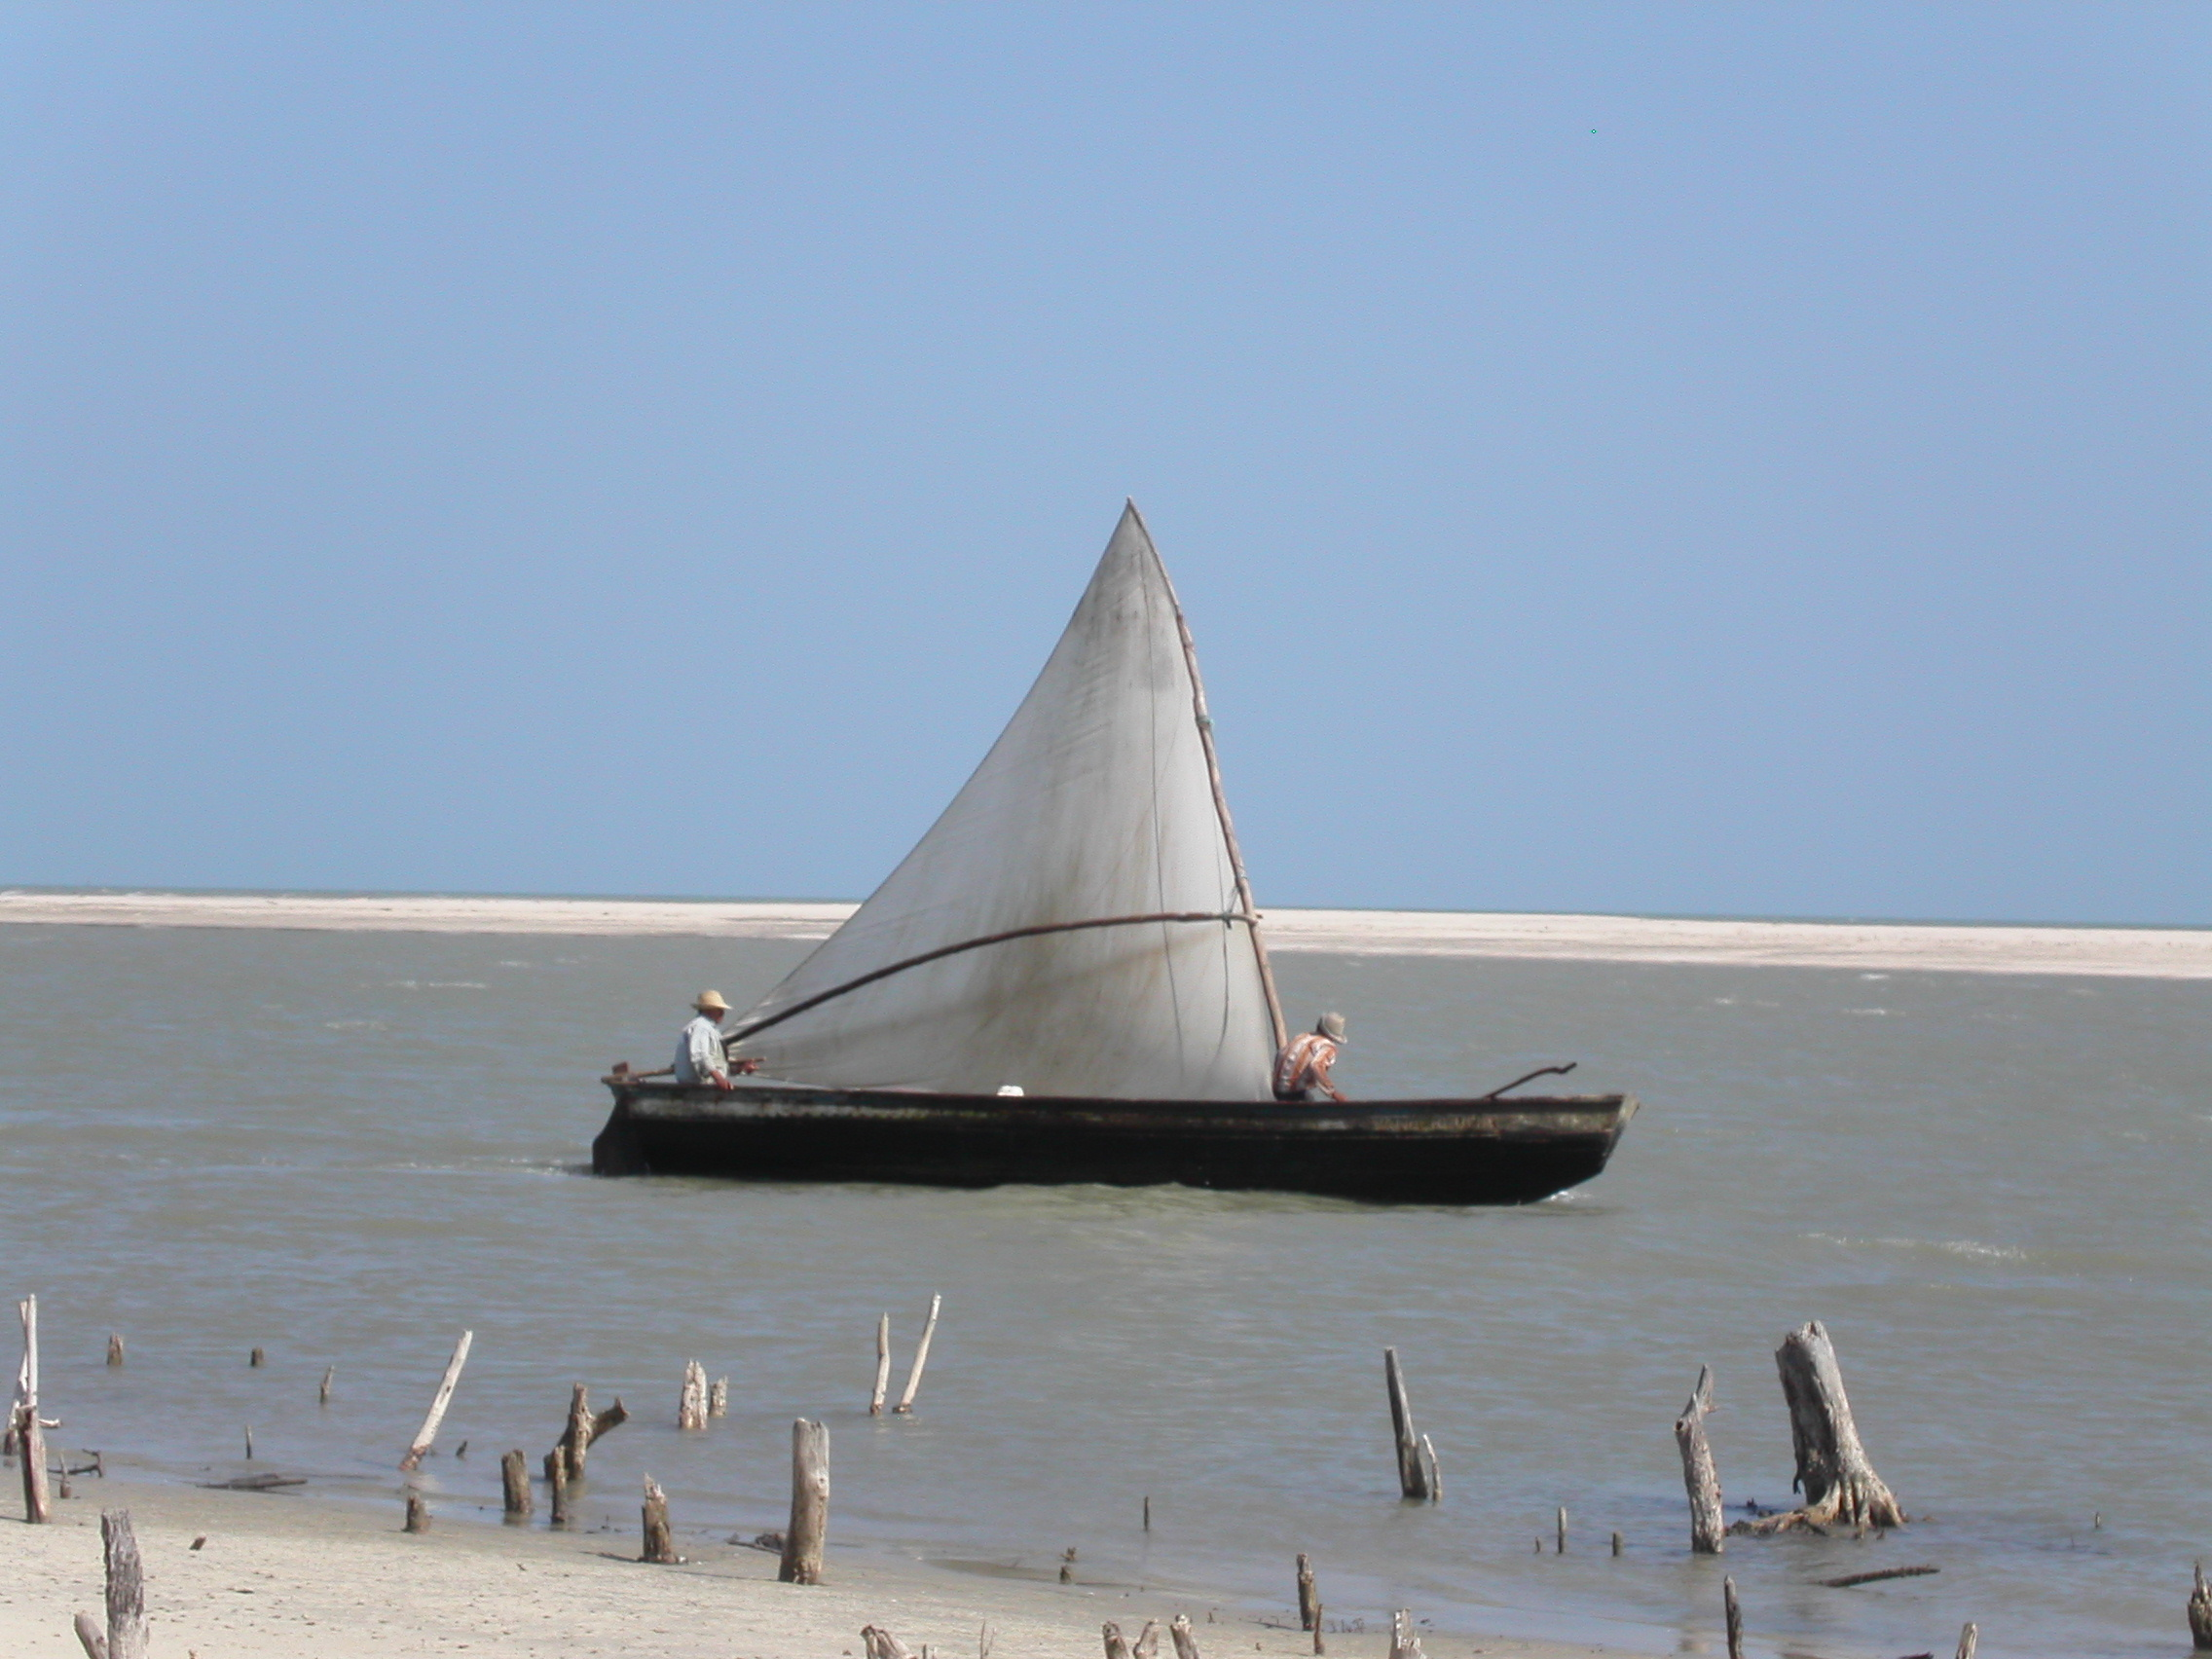
\includegraphics[width=0.75\textwidth]{../pictures/brasil.jpg}
\end{minipage}%
\begin{minipage}{0.5\textwidth}
\centering
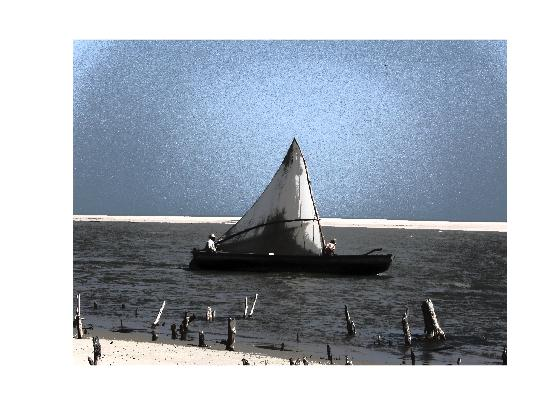
\includegraphics[width=0.98\textwidth]{images/p1_brasil.jpg}
\end{minipage}
\caption{\textit{Illustration de l'apparition de pixels nuisibles dûs à la ré-allocations de bits dans l'histogramme produisant une mauvaise quantification des couleurs.}}
\label{fig:p1_brasil}
\end{figure}

\begin{figure}[!htb]
\centering
\begin{minipage}{0.5\linewidth}
\centering
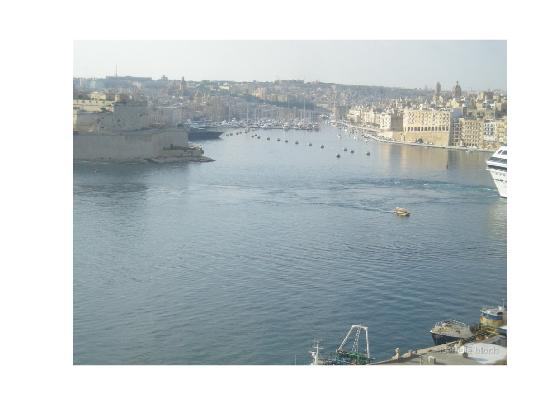
\includegraphics[width=0.98\linewidth]{images/im_x.jpg}
\end{minipage}%
\begin{minipage}{0.5\linewidth}
\centering
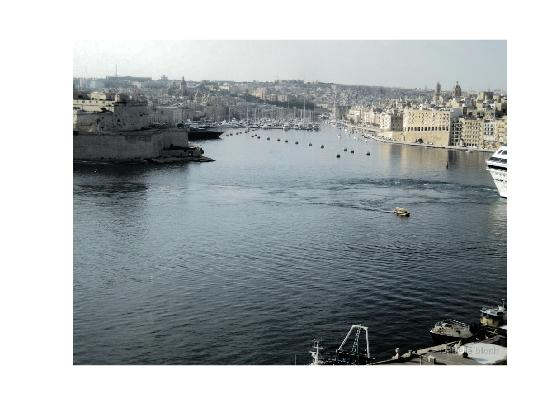
\includegraphics[width=0.98\linewidth]{images/im_xx.jpg}
\end{minipage}
\caption{\textit{Image de départ et son équivalent après spécification. On remarque qu'en haut à gauche, il y a des pixels apparents dans le ciel dûs à une mauvaise allocation des couleurs après spécification d'histogramme.}}
\label{fig:im_x}
\end{figure}

\begin{figure}[!hbt]
\centering
\begin{minipage}{0.33\textwidth}
\centering
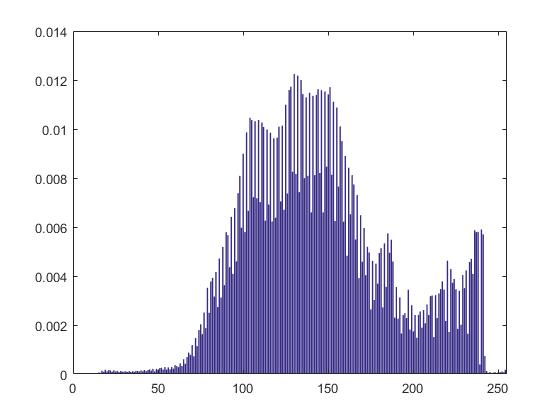
\includegraphics[width=0.98\textwidth]{images/hist_x.jpg}
\end{minipage}%
\begin{minipage}{0.33\textwidth}
\centering
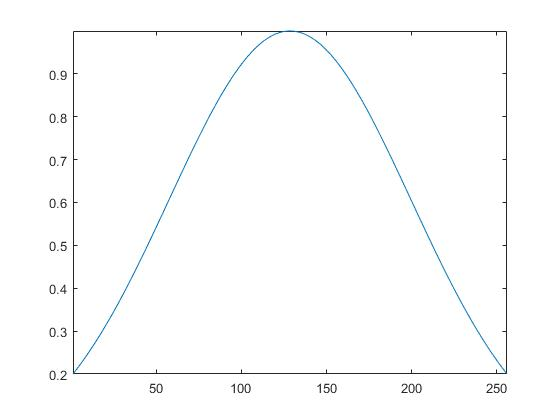
\includegraphics[width=0.98\textwidth]{images/p1_hist_cible_malte.jpg}
\end{minipage}%
\begin{minipage}{0.33\textwidth}
\centering
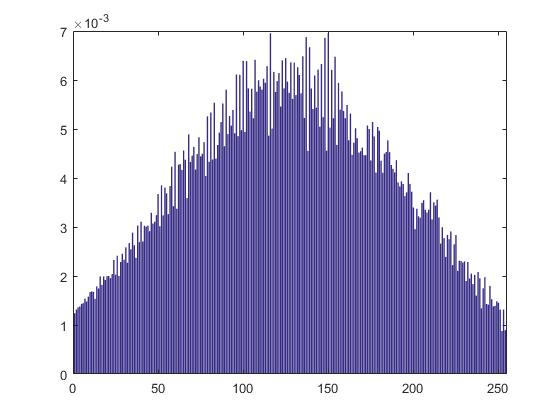
\includegraphics[width=0.89\textwidth]{images/hist_xx.jpg}
\end{minipage}
\caption{\textit{Gauche: histogramme de départ, Milieu: forme de l'histogramme cible, Droite: histogramme obtenu après application de la spécification par la routine order}}
\label{fig:im_xx}
\end{figure}
\FloatBarrier

\section{Divers pistes}
\paragraph*{}
Dans cette section, nous souhaitons faire part des différentes approches que nous avons entrepris pour résoudre le problème de "large pixel". 

\subsection{Approche par tilling}
Une première idée a été de vouloir traiter des bouts d'images indépendamment les uns des autres car le problème est souvent localisé dans certaines zones de l'image. Les approches par tilling et pyramides multi-échelles étant monnaie courante en traitement des image, nous avons voulu l'essayer dans notre problème. Malheureusement, qui dit tilling dit traitement séparé des informations ce qui ne nous arrange pas car nous voulons dispatcher l'ensemble des pixels de l'image et les réorganiser. Le résultat obtenu (sans utiliser d'algorithme type Midway qui aurait permis d'unifier les couleurs des différentes imagettes) n'est pas convaincant du tout car des zones claires et foncées apparaissent là où on le veut pas comme on peut le voir dans la figure \ref{fig:tilling} où les jonctions de chacune des imagettes pose problème. Cette figure a été obtenue avec une approche de type pyramide où chaque quart est la moyenne entre le quart de l'image de niveau 0 et l'imagette traitée à part au niveau 1 avec son propre histogramme (cf code dans le dossier "tilling").

\begin{figure}
\centering
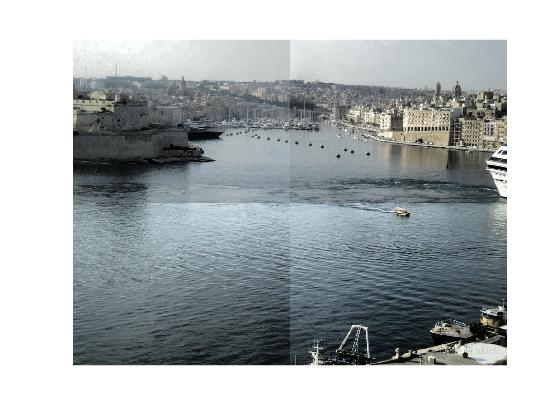
\includegraphics[scale=0.75]{images/p2_tilling.jpg}
\caption{\textit{Sans même se donner la peine de traiter l'image par un algorithme type midway pour unifier les couleurs, on aperçoit dans l'image en haut à droite que le ciel est un dégradé qui ne prend pas en compte le ciel de l'imagette en haut à gauche. Pire encore, le phénomène de "large pixels" est encore plus accentué car on a encore moins de bits à allouer aux zones claires ! Même constat pour chacune des jonctions.}}
\label{fig:tilling}
\end{figure}
\FloatBarrier

\subsection{Résolution par ajout de bruit}
\subsubsection*{Approche probabiliste}
La partie précédente met en évidence que le transport d'un histogramme d'une image réelle vers un histogramme cible ne peut se faire ni directement ni par découpes successives. On obtient toujours des défauts dans l'image générée à partir du nouvel histogramme.\\
Suivant nos idées initiales, nous sommes partis du constat qu'une image est la réalisation d'une variable aléatoire $X$ vivant dans un espace de très grande dimension (de l'ordre du million en pratique) et que son ou ses histogrammes, selon que X est une image couleur ou en niveau de gris, représentent les distributions de probabilités de chacun des canaux. Dans ce contexte, on peut utiliser un résultat classique de probabilités:
\paragraph*{Théorème 1:} Soient $x$ et $y$ les réalisations de deux variables aléatoires $X$ et $Y$ de densités respectives $f_x$ et $f_y$. Alors $x+y$ est aussi une variable aléatoire suivant la loi $X+Y$ et de densité $f_x * f_y$.\\

Toutes les considérations suivantes seront prises sur des images en niveaux de gris. Pour appliquer les résultats à des images couleurs, il suffit d'appliquer les calculs à chacun des canaux. On considérant maintenant que $x$ est notre image et en notant $b$ le bruit (gaussien, uniforme, peu importe), on obtient que l'image $x_b = x+b$ possède un histogramme qui s'écrit $h_x * h_b$. On peut donc maintenant jouer sur le type de bruit et son écart-type $\sigma$ pour modifier l'allure de l'histogramme  de $x$ et donc modifier en aval le contraste de manière plus fine.\\
Théoriquement, on arrive alors a moyenner l'histogramme de x. On définit la valeur d'un bin $h_{x_b}(i)$ pour $i \in {0,...,255}$ comme une fonction de de $h_x(i)$ mais aussi de ses voisins. On force donc l'histogramme a avoir des valeurs faibles aux endroits où il n'y avait pas de pixels au départ et où l'algorithme faisait apparaitre beaucoup de pixels. Cela  réduit l'apparition de problèmes de larges pixels. Le choix du type de bruit à appliquer définit aussi le type de moyenne que l'on utilise. Par exemple un bruit uniforme appliquera une moyenne classique aux bins de l'histogramme de $x$.

\subsection{Méthodes de dithering}
\paragraph*{}
L'idée d'ajouter du bruit à l'image pour casser ces zones constantes n'est pas nouvelle et date du milieu des années 50. Entre temps, le domaine de la quantification des palettes de couleurs a connu un grand intérêt avec l'arrivée des écrans couleurs. La trame de Bayer est l'un des exemples les plus connus, permettant de coloriser par des hachures des images. Globalement cette technique fonctionne bien mais fait apparaître des artefacts dans les zones hautes-fréquences. Notre problème étant celui de traiter de coloriser des zones de teinte constante qui deviennent à teinte variable après application de l'algorithme. La littérature à ce sujet est assez riche et plusieurs algorithmes sont disponibles comme celui de Floyd et Steinberg de 1975. Nous avons choisi l'algorithme d'Atkinson datant des années 80 qui repose sur la technique de Floyd et Steinberg mais est plus rapide et donne de meilleurs résultats.
\subparagraph*{}
Le principe de ces algorithmes est assez simple. Pour chaque pixel codé, on attribut une valeur $q_i$ appartenant aux valeurs de quantifications possibles $q_j$, $\forall j \in {1,..., L}$ puis on garde en mémoire l'erreur entre cette valeur quantifiée $q_i$ et la véritable valeur de ce pixel. On la propage aux pixels voisins et on quantifie la valeur voisine en ajoutant l'erreur de quantification du premier pixel ce qui permet de créer des structures en damier ou des sortes de patchworks plus ou moins denses de pixels noirs et blancs pour donner l'impressions de plusieurs teintes de gris alors qu'on a que deux couleurs. Dans le cas des images couleurs, le procédé est appliqué à chacun des canaux de couleurs.
\subparagraph*{}
Avec cette procédure simple mais astucieuse, on arrive à gommer beaucoup des erreurs de quantifications. L'idée du procédé n'est pas étrangère à notre première approche du problème car même si nous avons pensé en terme d'histogramme au début, ajouter du bruit revient à casser la redondance des zones constantes et donc à donner un aspect plus contraster et moins bloc de couleurs dans les zones unis, les zones hautes-fréquences ne faisant pas ressortir le grain du bruit.

\subsection{Résolution par étude de la fonction de répartition}
\paragraph*{}
Une approche plus en lien avec le papier expliquant la construction de la méthode de tri et d'ordonnancement est de s'intéresser à la fonction de répartition de l'image. Le code de base fournit une fonction pour obtenir un histogramme cible à partir d'une gaussienne. Dans le cas de l'image du bungalow \ref {fig:bungalow}, le résultat est très bon. En adaptant les bornes $L$ et $R$ de la fonction, on peut trouver de bons résultats pour des images dont la fonction de répartition est relativement simple (aucun point d'inflexion, allure d'une fonction de répartition d'une gaussienne, comportement très régulier...).La figure \ref{fig:histograms} illustre ce constat. Il suffit de voir le résultat sur l'image "Malta" \ref{fig:malta} où on n'aperçoit plus du tout les "large pixels" une fois les bons paramètres $L$ et $R$ trouvés ($L = 0.2$, $R = 0.5$).

\begin{figure}[!hbt]
\centering
\begin{minipage}{0.5\textwidth}
\centering
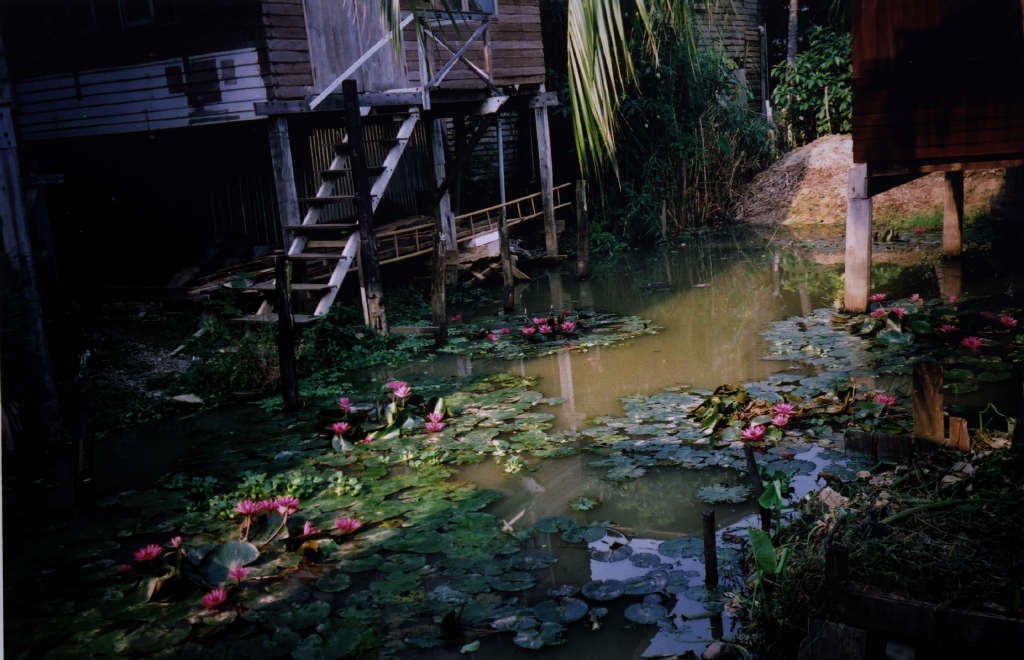
\includegraphics[width=0.77\textwidth]{../pictures/bungalow.png}
\end{minipage}%
\begin{minipage}{0.5\textwidth}
\centering
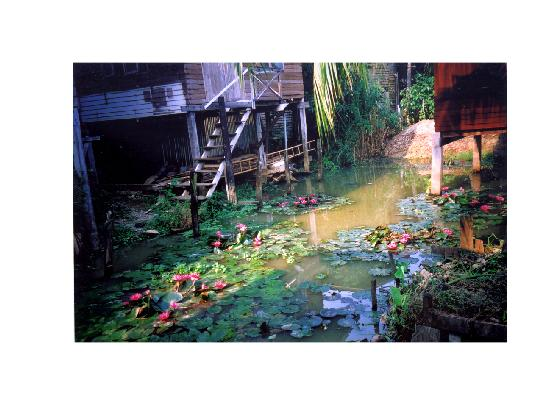
\includegraphics[width=0.98\textwidth]{images/p3_bungalow_xx.jpg}
\end{minipage}
\caption{\textit{Cas où tout se passe bien, celui de l'image de bungalow.}}
\label{fig:bungalow}
\end{figure}

\begin{figure}[!hbt]
\centering
\begin{minipage}{0.33\textwidth}
\centering
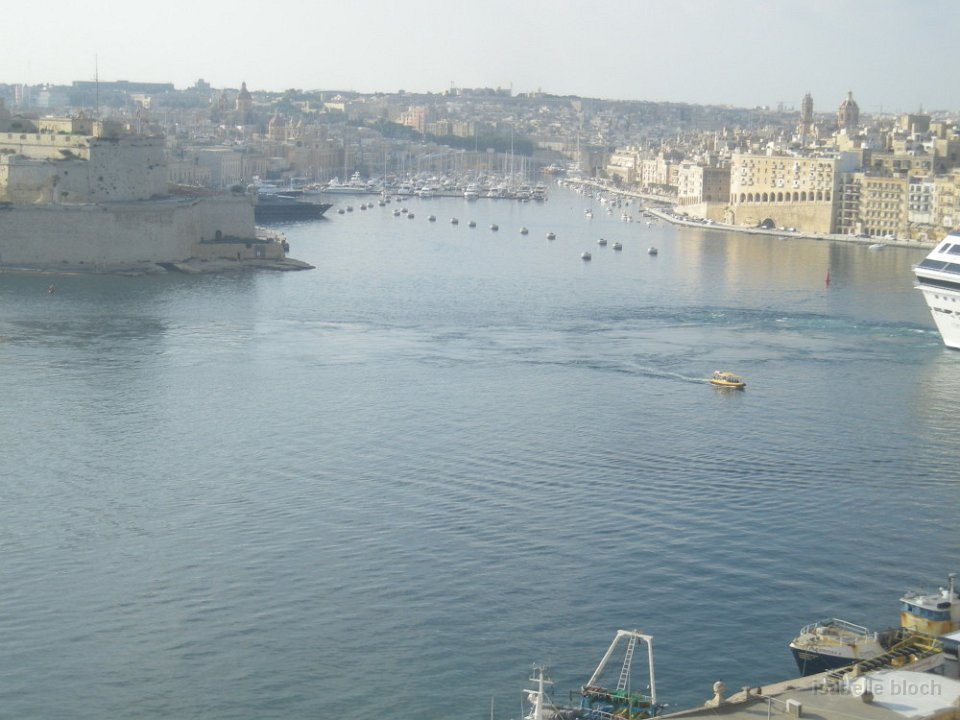
\includegraphics[width=0.77\textwidth]{../pictures/Malta.JPG}
\end{minipage}%
\begin{minipage}{0.33\textwidth}
\centering
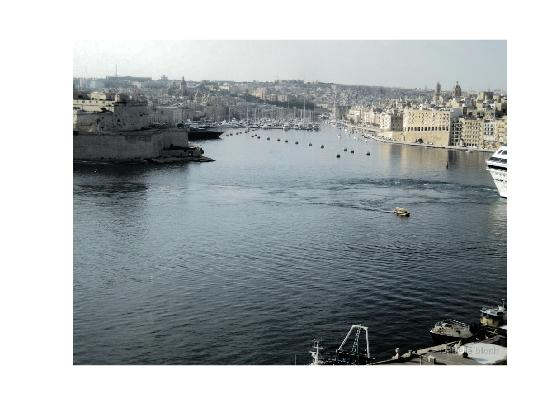
\includegraphics[width=0.98\textwidth]{images/im_xx.jpg}
\end{minipage}%
\begin{minipage}{0.33\textwidth}
\centering
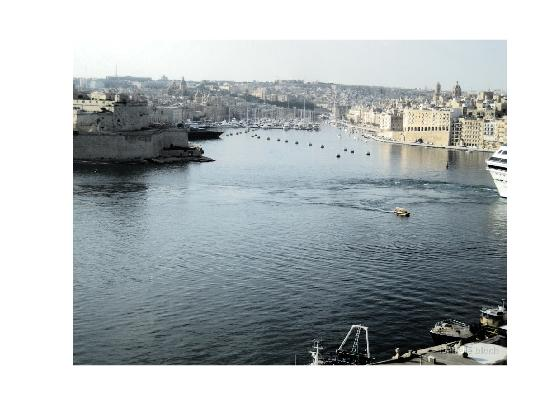
\includegraphics[width=0.98\textwidth]{images/p3_malta_xx.jpg}
\end{minipage}
\caption{\textit{A gauche, l'image de départ, au milieu, l'image obtenue avec une gaussienne répartissant mal les pixels et à droite image obtenue avec un choix de gaussienne plus judicieux qui distribue plus de pixels dans les zones clairs pour améliorer l'allure du dégradé.}}
\label{fig:malta}
\end{figure}

\begin{figure}[!hbt]
\centering
\begin{minipage}{0.25\textwidth}
\centering
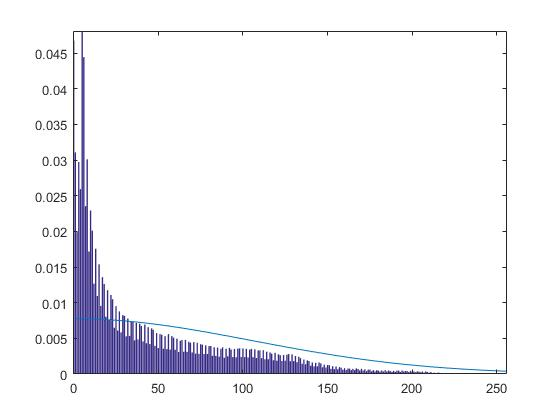
\includegraphics[width=0.98\textwidth]{images/p3_bungalow_hist.jpg}
\end{minipage}%
\begin{minipage}{0.25\textwidth}
\centering
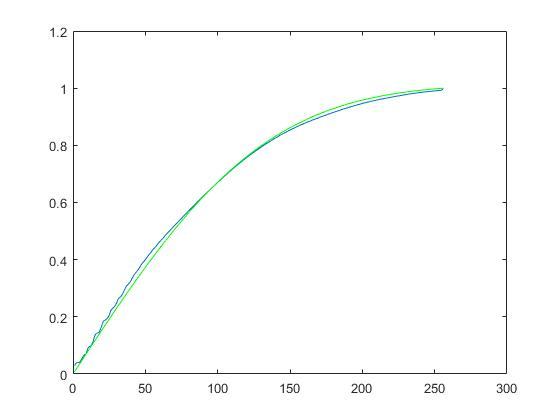
\includegraphics[width=0.98\textwidth]{images/p3_bungalow_cumsum.jpg}
\end{minipage}%
\begin{minipage}{0.25\textwidth}
\centering
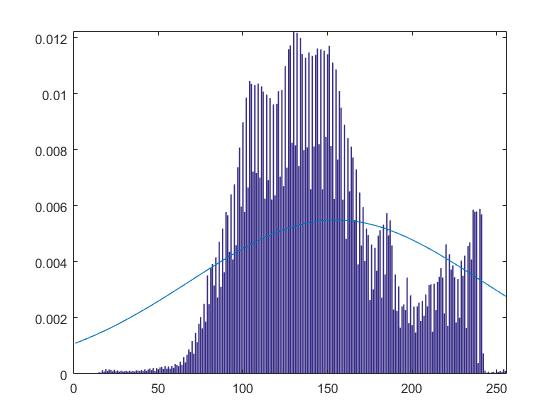
\includegraphics[width=0.98\textwidth]{images/p3_malta_hist.jpg}
\end{minipage}%
\begin{minipage}{0.25\textwidth}
\centering
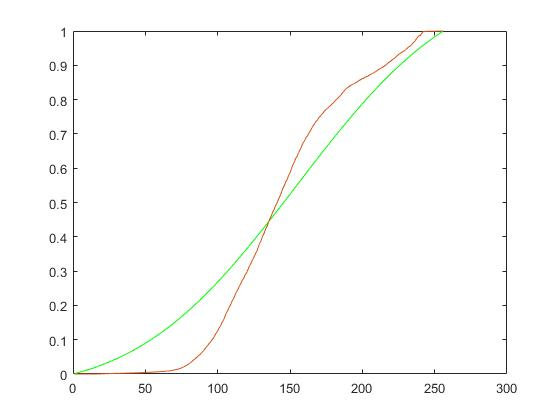
\includegraphics[width=0.98\textwidth]{images/p3_malta_cumsum.jpg}
\end{minipage}
\caption{\textit{A gauche, histogrammes et histogrammes cumulés pour la photo du bungalow et à droite, la même chose pour la photo de Malte. Dans le cas du bungalow, on trouve un histogramme qui permet une spécification exacte comme expliqué dans l'article. Dans le cas de Malte, on trouve un fonction approché, mais qui donne un résultat très satisfaisant.}}
\label{fig:histograms}
\end{figure}
\FloatBarrier
\subsection*{Optimisation des paramètres}
Le but est alors de trouver la fonction modélisant le plus finement l'histogramme de départ. Nous avons utilisé la routine hsGauss.m pour coller au mieux à l'histogramme de départ tout en distribuant des pixels sur toute l'amplitude de niveaux de gris allant de 0 à 255. Il faut donc jouer sur les paramètres $R$ et $L$ qui définissent la gaussienne cible. On tombe sur un problème de "curve fitting" qui peut s'écrire (h désigne l'histogramme de départ et g la gaussienne obtenue par hsGauss):
\begin{equation}
\min_{(L, R)} ||h - g(L, R)||^2
\end{equation} 
Comme $L$ et $R$ sont compris entre 0 et 1, on doit ajouter quatre contraintes inégalités au problème. Si on pose $u=(L,R)$, alors on a $h_1(u) = -L$, $h_2(u) = L-1$, $h_3(u) = -R$ et $h_4(u) = R-1$. Le problème s'écrit alors avec les $\lambda_i$ des réels positifs:
\begin{equation}
\min_{u} ||h - g(u)||^2 + \sum_{i=1}^4 \lambda_i h_i(u)
\end{equation} 
\paragraph*{}
On a réussi à poser correctement le problème sous la forme d'un problème d'optimisation quadratique sous contraintes. Un tel problème peut se résoudre par la méthode d'Uzawa par exemple et le code utilisé se situe dans le dossier \textit{optim\_R\_L} du code. Malheureusement comme nous le verrons dans l'exemple suivant, l'optimisation des paramètres ne suffit pas à effacer les problèmes de large pixels.
\pagebreak
\subsection*{Limite de la méthode}
En effet, Pour des images où la répartition du contraste est beaucoup plus localisé et que l'on a plusieurs clusters de niveaux de gris par exemple, la modélisation par une gaussienne dessinée à la main ou optimisée est trop grossière comme le montre la figure \ref{fig:birds}. On remarque sur l'histogramme cumulé la présence de deux paliers atteints qui correspondent à la présence de deux pics dans l'histogramme. Dans ces conditions, une approximation gaussienne ne permet pas d'imiter ce comportement. C'est le cas pour l'image des oiseaux par exemple. Le fond étant presque uni et clair, un histogramme cible gaussien va avoir tendance à redistribuer trop largement les pixels et faire apparaitre des dégradés sur l'image synthétique, c'est un problème analogue aux larges pixels.


\begin{figure}[!hbt]
\centering
\begin{minipage}{0.25\textwidth}
\centering
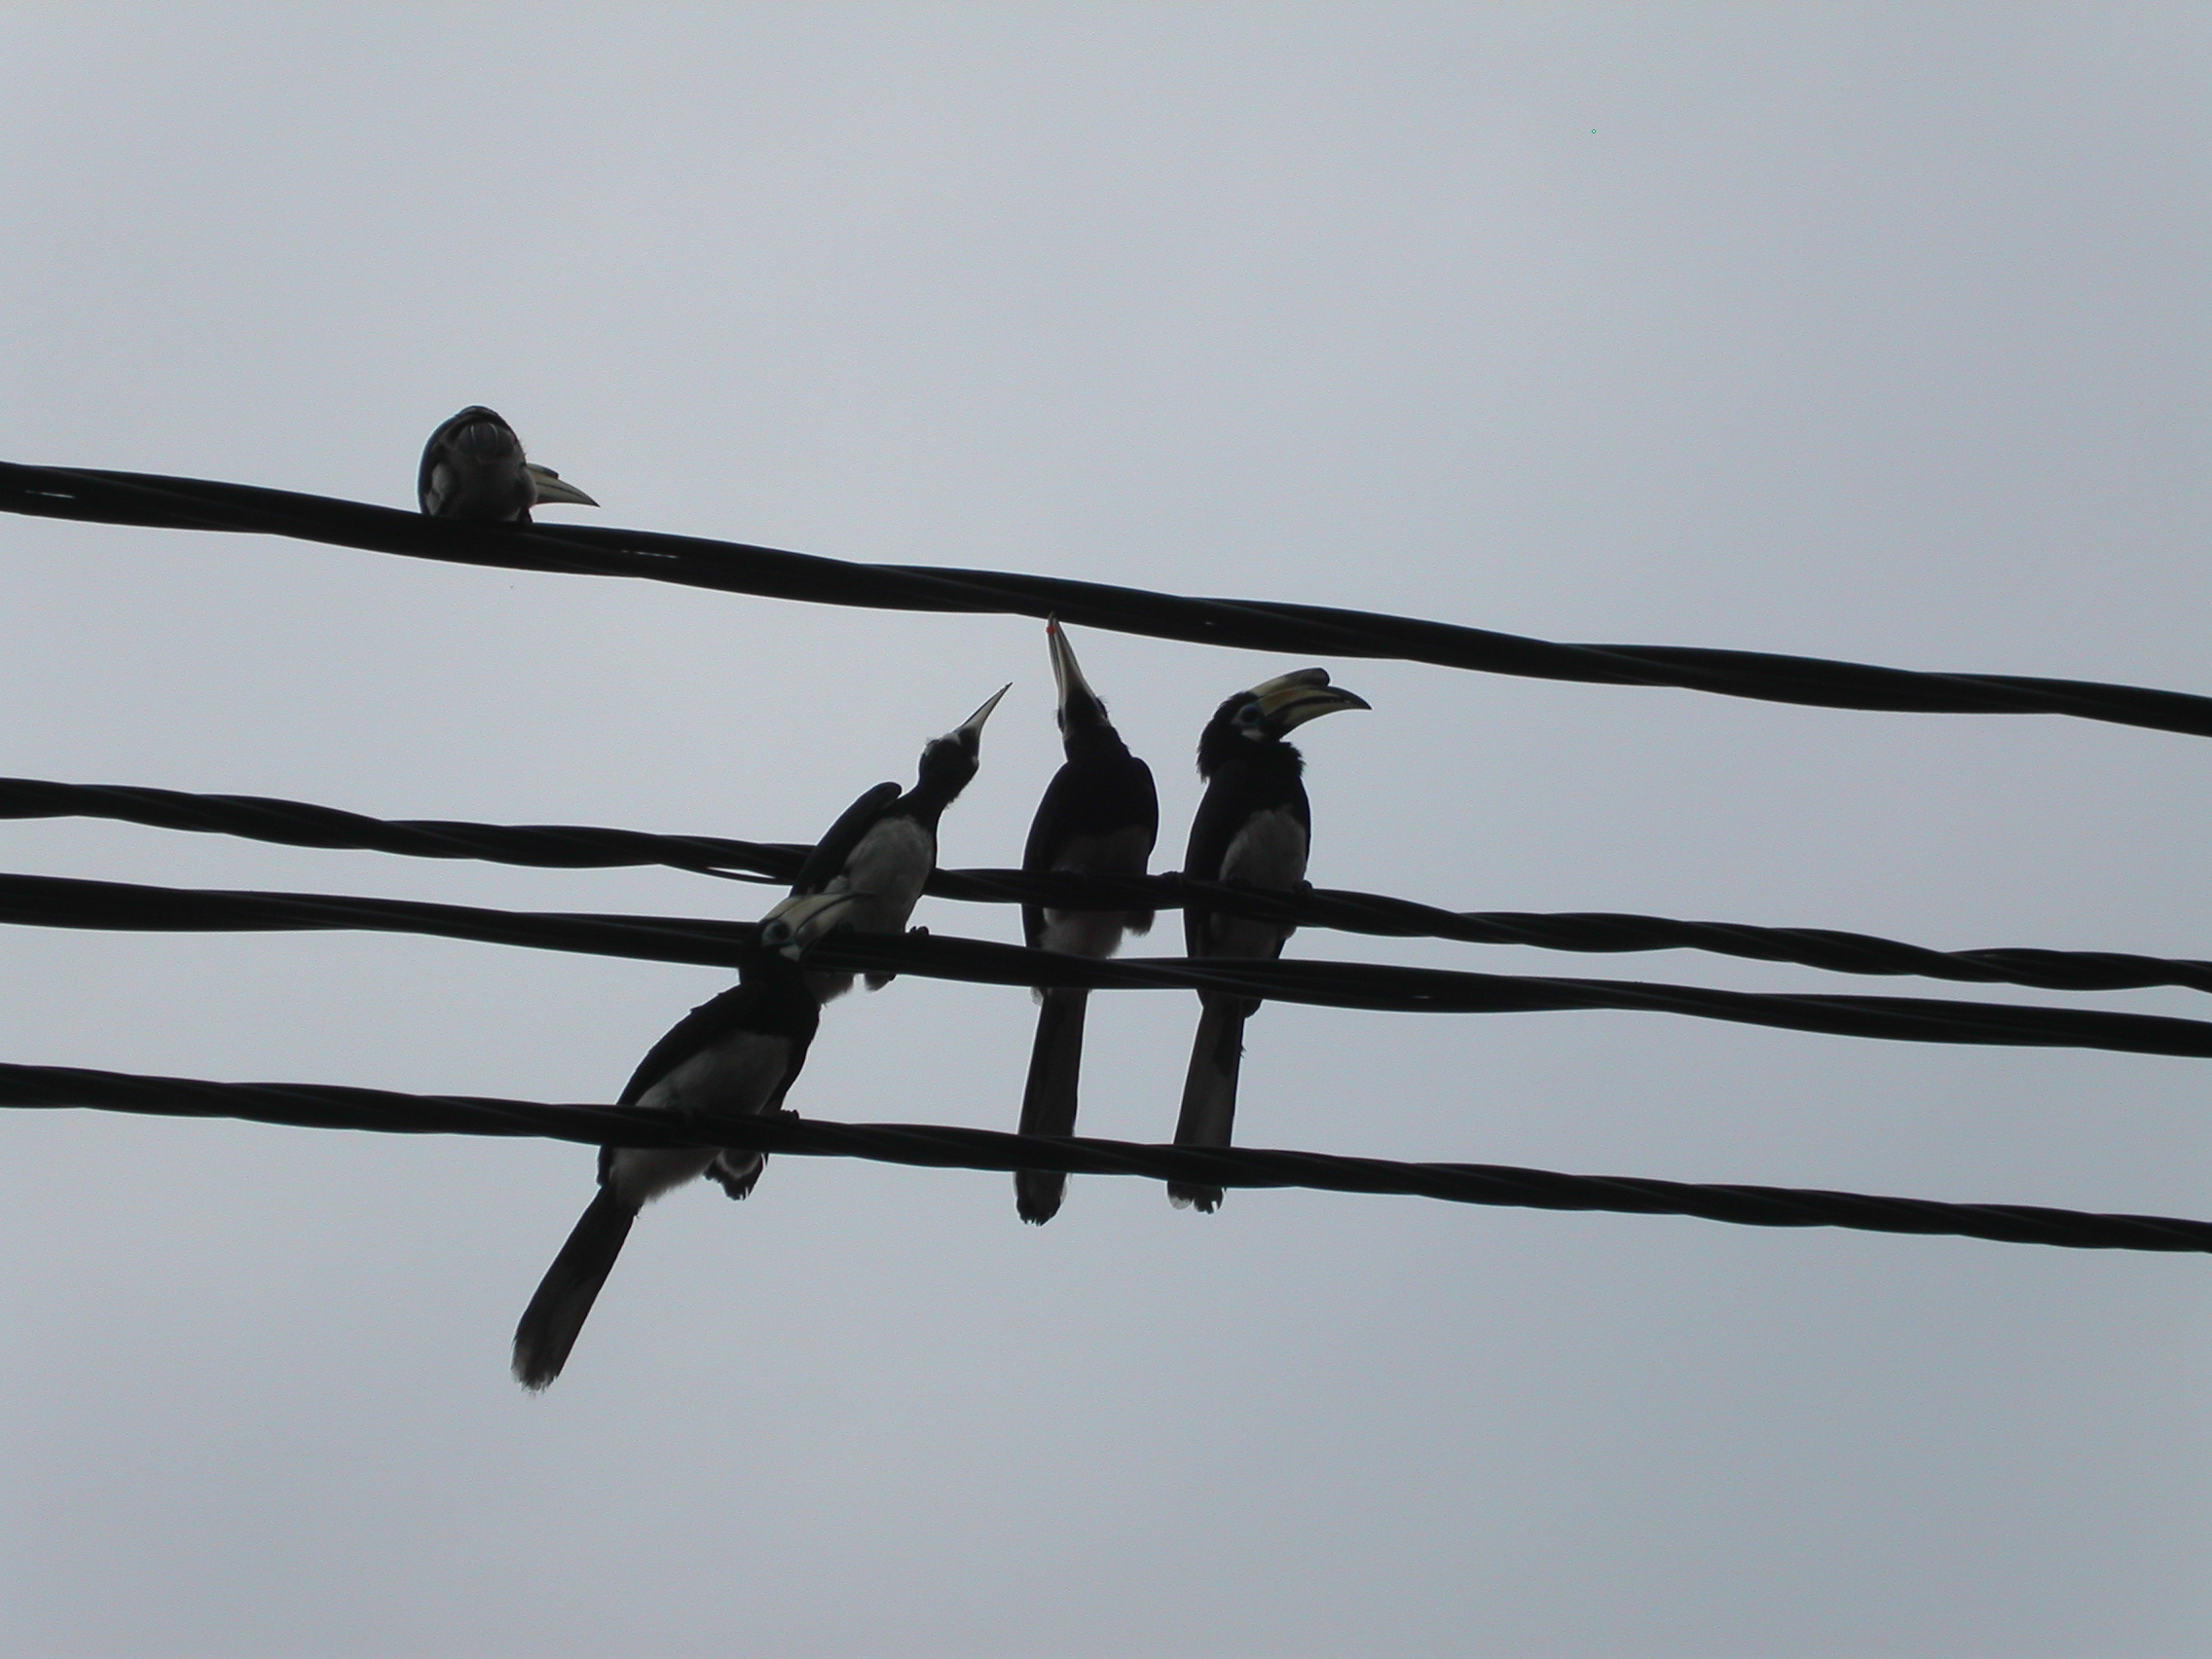
\includegraphics[width=0.77\textwidth]{../pictures/birds.jpg}
\end{minipage}%
\begin{minipage}{0.25\textwidth}
\centering
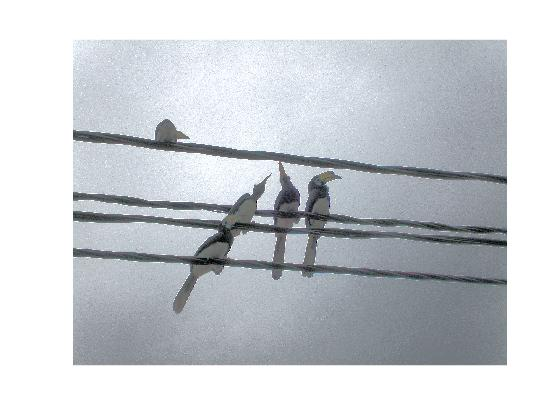
\includegraphics[width=0.98\textwidth]{images/p3_birds_xx.jpg}
\end{minipage}%
\begin{minipage}{0.25\textwidth}
\centering
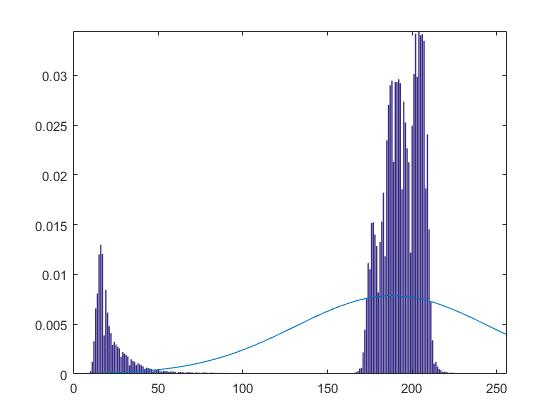
\includegraphics[width=0.98\textwidth]{images/p3_birds_hist.jpg}
\end{minipage}%
\begin{minipage}{0.25\textwidth}
\centering
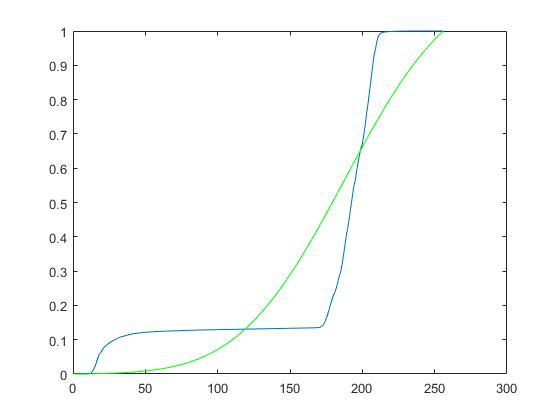
\includegraphics[width=0.98\textwidth]{images/p3_birds_cumsum.jpg}
\end{minipage}
\caption{\textit{De gauche à droite: l'image originale, l'image "améliorée", l'histogramme de l'image de départ et la fonction cible et les fonctions de répartition associées.On remarque que le bord supérieur droit est moins sombre dans la dernière image, conséquence de l'allocation des pixels en faveur des zones claires.}}
\label{fig:birds}
\end{figure}
\FloatBarrier
Une idée supplémentaire serait d'avoir une fonction pas trop régulière car celle-ci risquerait d'allouer trop de pixels à des bins non présents sur l'image d'origine.On peut alors imaginer trouver des fonctions plus compliquées que la gaussienne qui régularisent l'histogramme cumulé et qui s'adaptent aux problèmes de sauts brusques dans la fonction de répartition. Cependant, même en trouvant de telles fonctions, d'autres histogrammes cibles poseront sûrement problème et il faudrait alors trouver un autre type de fonction qui approximerait l'histogramme cible.

\section{Suppression des larges pixel par TMR}
Nous avons vu que par l'approximation de l'histogramme par une gaussienne puis l'application de l'algorithme de \textit{ranking} nous obtenons deux types de résultats. Soit le résultat est satisfaisant car l'histogramme de base peut facilement être approximé par une gaussienne, soit la forme de l’histogramme est très éloigné d'une gaussienne et la redistribution des pixels fait apparaître (le plus souvent dans les zones d’aplats de couleur)  le problème des larges pixels.  Dans cette partie nous présentons une solution qui combine deux approches: approximation de l'histogramme par une somme de gaussiennes puis nous appliquons un algorithme TMR tel que définit dans \cite{rabin:hal-00505966} pour faire disparaître les large pixels. On rappelle ici l'algorithme en question qui permet de réadapter les contrastes d'une image spécifiée pour que les artefacts de celle-ci disparaissent.
\begin{equation}
TMR_u[(g(u)] = u+Y_u[g(u)-u] = Y_u[g(u)] + u-Y_u[u]
\end{equation}
Où $u$ est l'image de départ, $g(u)$ est l'image spécifiée et $Y_u[w](x) = \frac{1}{C(x)} \sum_{y \in \mathcal{N}(x)}w(y)e^{\frac{||u(x)-u(y)||^2}{\sigma^2}}dy$ est le filtre guidé. On répète $N$ fois cette opération pour

\subsection{Détection de pics et choix de la forme de l'histogramme cible}
\subsubsection{Détection des pics}
En se basant sur le code \textit{hsGauss.m} nous avons écrit une fonction qui permet de repérer les pics sur l'histogramme et de fitter la meilleure gaussienne dessus. Dans un deuxième temps nous avons rajouté un calcul de l'écart type autour de ce pic pour choisir entre fitter une gaussienne ou une laplacienne qui correspond à un pic plus étroit adaptant encore plus l'histogramme cible à celui de départ mais les résultats ne sont pas plus concluants qu'avec un de choix de gaussiennes et il est préférable de sélectionner la forme de cette dernière pour conserver l'aspect "étalement des bits" sur tout l'histogramme. L'histogramme que nous obtenons en sortie est le maximum point par point des gaussiennes fitter sur chaque pic, pondéré en fonction de la hauteur de celui-ci. Nous avons aussi choisi d'adapter les paramètres L et R des scripts \textit{hsGauss.m} et \textit{hsLaplace.m} en fonction de la position du maximum local détecté. Ainsi nous avons choisi de subdivise l'espace des valeurs de pixels en 5 segments de longueur à peu près égales. En pratique nous avons adapter des paramètres L et R selon que le bon se situe dans [0, 50], (50, 100], (100, 150], (150, 200] et (200, 255] ce qui permet de coller grossièrement à l'histogramme de départ. Ceci rejoint notre tentative précédente d'optimiser sur L et R en résolvant un problème de curve-fitting. Cette simplification de la recherche L et R est un gain de temps énorme, une simplification de l'algorithme et en pratique donne d'excellents résultats.


\begin{figure}
\centering
\begin{minipage}{0.5\textwidth}
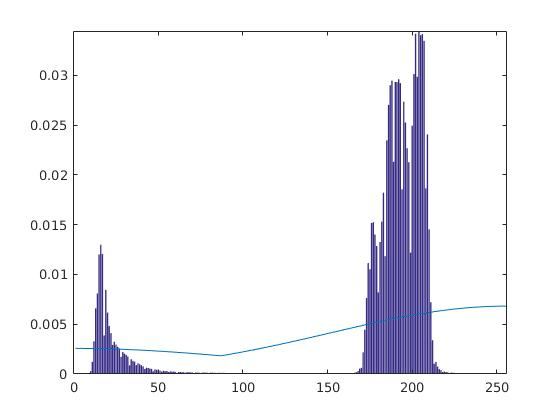
\includegraphics[scale=0.45]{images/birds_tmr_hist.jpg}
\end{minipage}%
\begin{minipage}{0.5\textwidth}
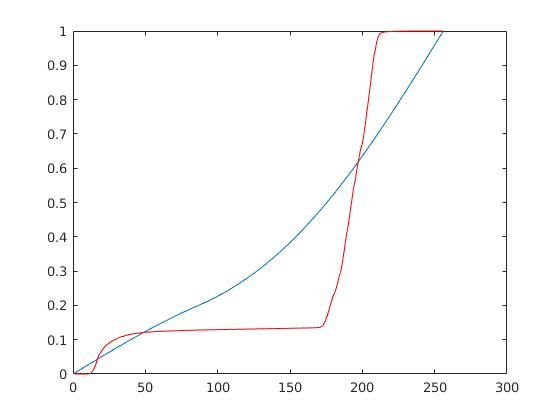
\includegraphics[scale=0.45]{images/cum_hist_bird.jpg}
\end{minipage}

\caption{\textit{Notre algorithme a reconnu deux pics et dessine l'histogramme cible comme étant le maximum point par point des deux gaussiennes fittées sur chaque pic. En rouge, l'histogramme cumulé de départ et en bleu notre nouvel histogramme.}}
\label{fig:choosehs}
\end{figure}
\FloatBarrier

Comme nous pouvons le voir dans la figure \ref{fig:choosehs},  nous avons rajouté un paramètre dans notre fonction \textit{choosehsGauss.m} pour que deux pics trop rapprochés ne s'ajoutent pas dans le modèle.  Ainsi, nous considérons qu'un bin est un pic lorsque celui ci est éloigné au moins de 50 bins de tous les pics précédemment repérés. C'est un choix totalement arbitraire mais qui en pratique fonctionne bien. Le résultat de notre méthode pour l'image bird dont l'histogramme de la figure \ref{fig:choosehs} en est la répartition des pixels se trouve en figure \ref{fig:bird_tmr}.

\begin{figure}
\centering
\begin{minipage}{0.5\textwidth}
\centering
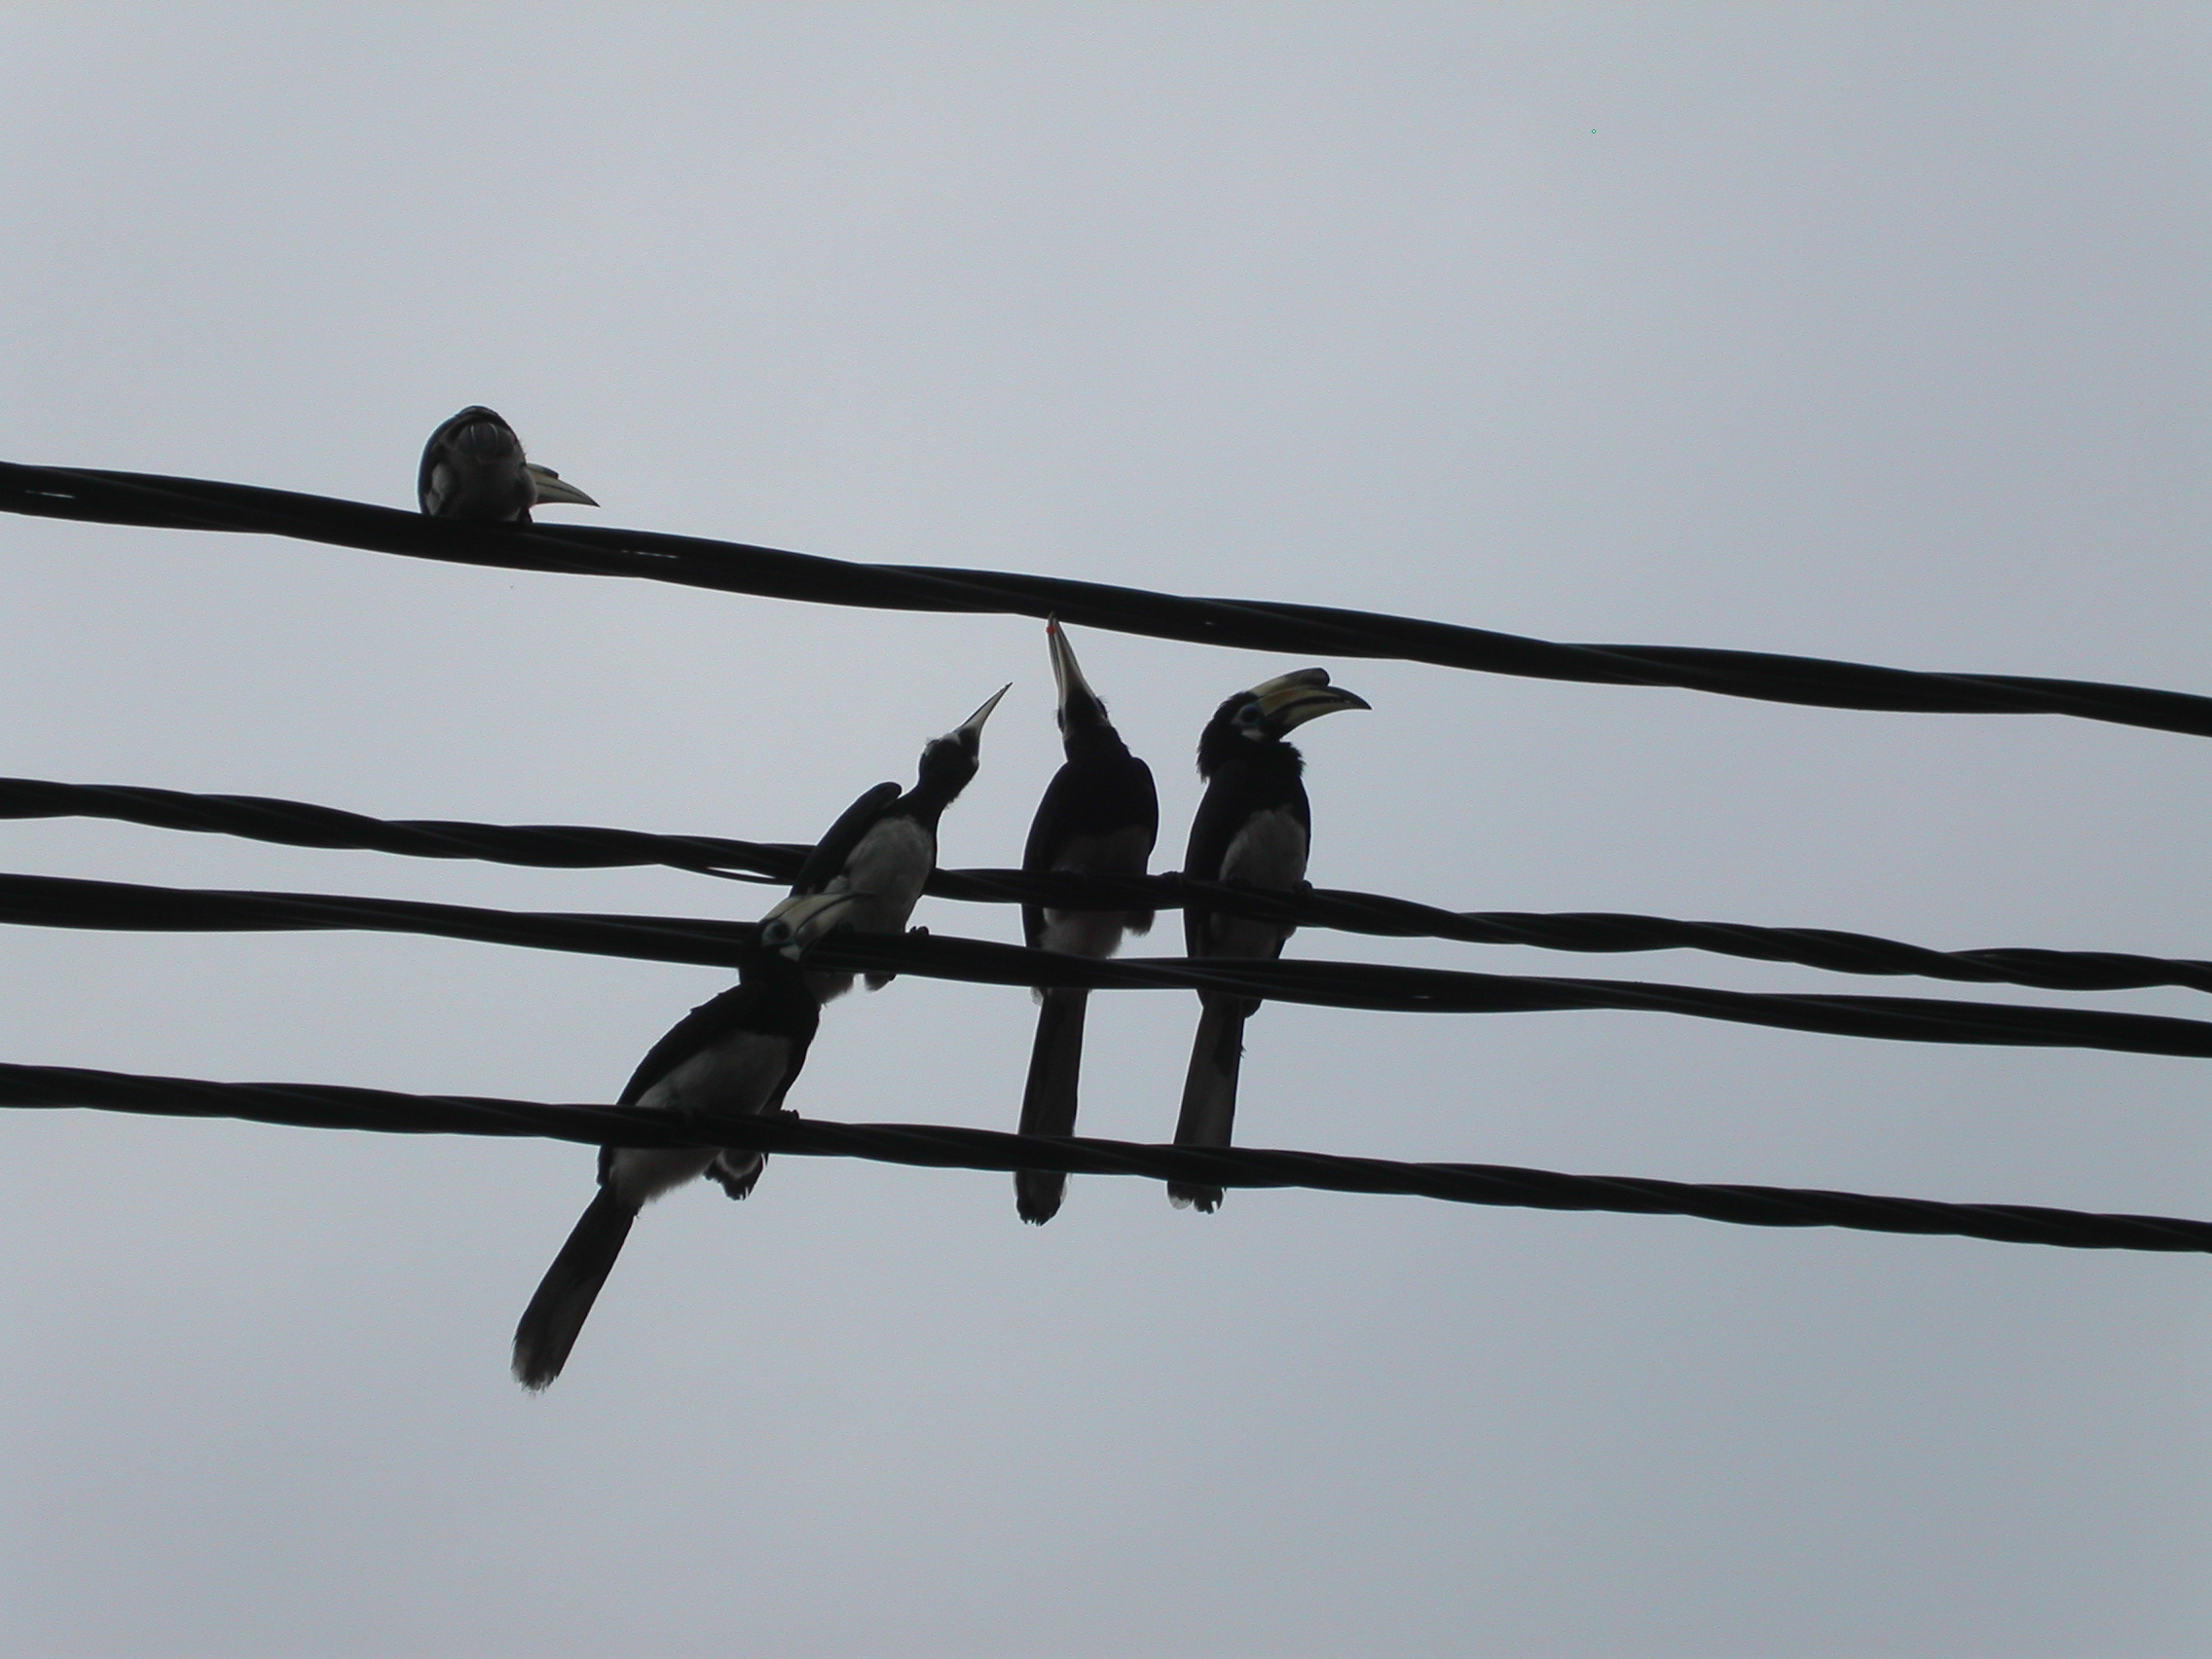
\includegraphics[width=0.8\textwidth]{../pictures/birds.jpg}
\end{minipage}%
\begin{minipage}{0.5\textwidth}
\centering
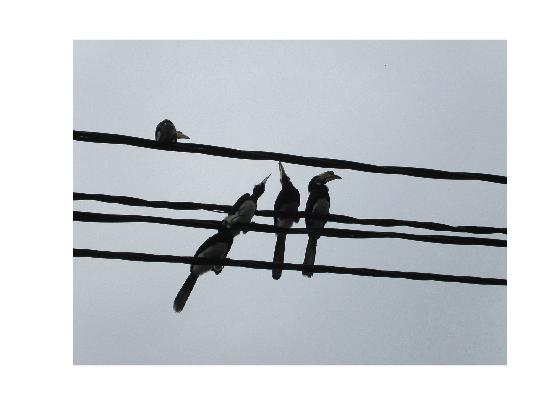
\includegraphics[width=1\textwidth]{images/birds_tmr.jpg}
\end{minipage}
\caption{\textit{A gauche, l'image modifiée par l'algorithme de base, A droite, sa version corrigée par notre algorithme mêlant curve fitting et TMR. On remarque bien que notre méthode gomme très bien les défauts visibles à gauche tout en respectant le ton neutre du ciel.}}
\label{fig:bird_tmr}
\end{figure}

Dans l'algorithme TMR, le choix d'un paramètre $\sigma$ détermine la taille de la fenêtre du patch qu'on doit restaurer. Pour des choix autour de 1, notre algorithme réagit très bien. La figure \ref{fig:malta_sigma} monter que pour plusieurs choix de ce paramètre autour de 1, des résultats plus ou moins satisfaisants sont visibles.

\begin{figure}
\centering
\begin{minipage}{0.33\textwidth}
\centering
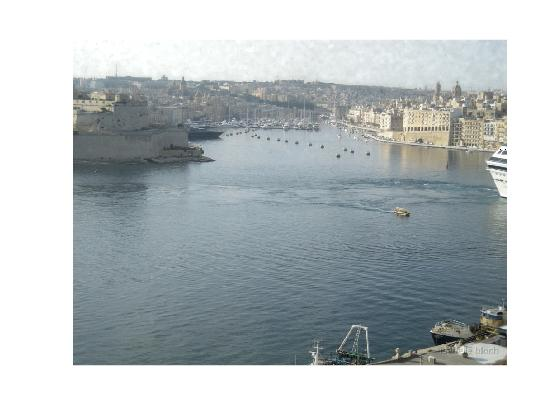
\includegraphics[scale=0.3]{images/malta_sigma_8.jpg}
\end{minipage}%
\begin{minipage}{0.33\textwidth}
\centering
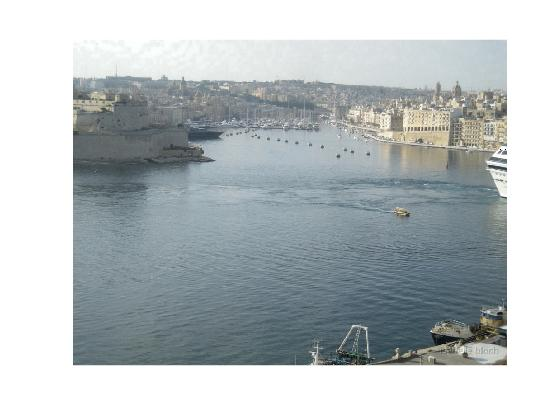
\includegraphics[scale=0.3]{images/malta_sigma_10.jpg}
\end{minipage}%
\begin{minipage}{0.33\textwidth}
\centering
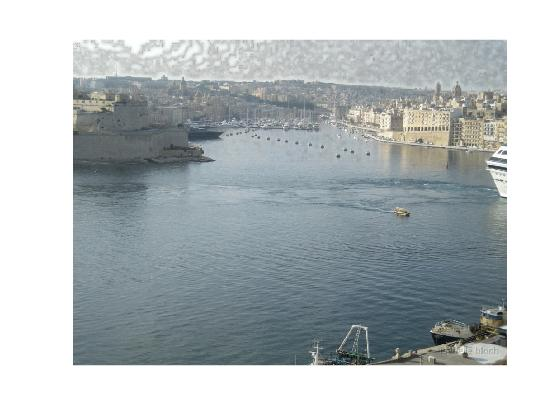
\includegraphics[scale=0.3]{images/malta_sigma_15.jpg}
\end{minipage}
\caption{\textit{De gauche à droite, $\sigma$ vaut 0.8, 1 et 1.5. Le paramètre $\sigma$ est primordial pour obtenir un bon résultat.}}
\end{figure}


\section*{Limitations de notre méthode}
Comme on peut le voir sur certaines images en Annexe A, notre méthode fonctionne globalement bien sur les images de test mais pour certaines, le changement de contraste n'est pas flagrant. L'algorithme de TMR semble détruire le changement de contraste en ramenant l'image modifiée vers l'image de départ.


\section*{Conclusion}
\paragraph*{}
Dans ce projet, nous avons donc cherché à résoudre le problème des larges pixels en jouant très fortement sur l'histogramme.\\
Notre première idée d'ajouter du bruit sur l'image s'est révélée être un bon point de départ. Fitter l'histogramme avec la meilleure gaussienne a permis de trouver qu'il fallait jouer sur le nombre de pics présents pour adapter au mieux le code donné. Enfin l'application de l'algorithme TMR à l'image obtenue par spécification de notre histogramme permet d'obtenir globalement des résultats très convaincants. 

\bibliographystyle{plain}
\bibliography{biblio}

\newpage
\section*{Annexe A: Quelques exemples de notre méthode}

\begin{figure}[h]
\centering
\begin{minipage}{0.33\textwidth}
\centering
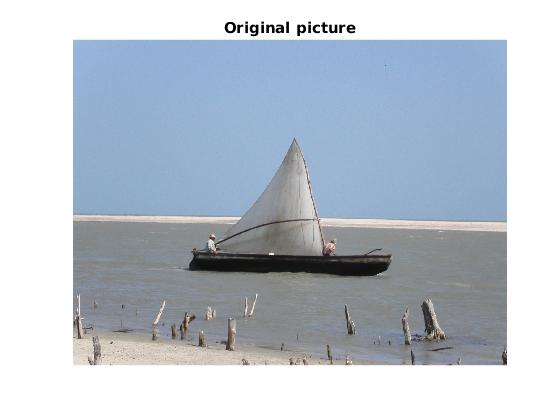
\includegraphics[width=1\textwidth]{images/boat_conc_depart.jpg}
\caption{Original}
\end{minipage}%
\begin{minipage}{0.33\textwidth}
\centering
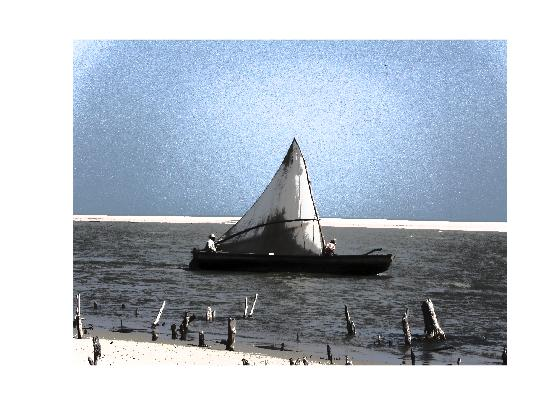
\includegraphics[width=1\textwidth]{images/boat_conc_inter.jpg}
\caption{Naïf}
\end{minipage}%
\begin{minipage}{0.33\textwidth}
\centering
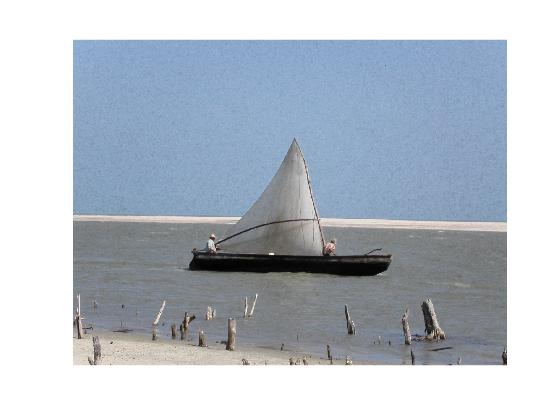
\includegraphics[width=1\textwidth]{images/boat_conc_tmr.jpg}
\caption{Le notre}
\end{minipage}
\end{figure}

\begin{figure}[h]
\centering
\begin{minipage}{0.33\textwidth}
\centering
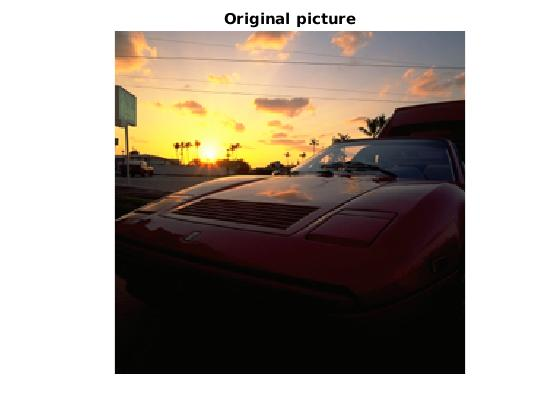
\includegraphics[width=1\textwidth]{images/ferrari_conc_depart.jpg}
\caption{Original}
\end{minipage}%
\begin{minipage}{0.33\textwidth}
\centering
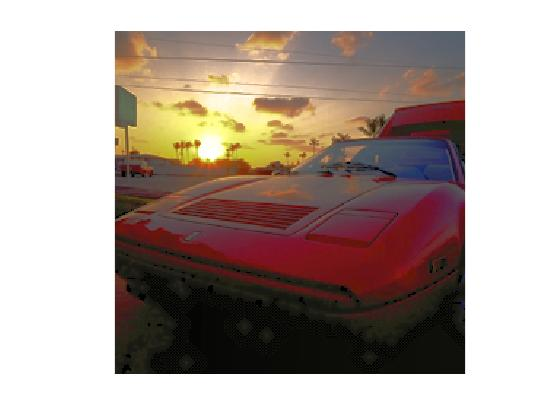
\includegraphics[width=1\textwidth]{images/ferrari_conc_inter.jpg}
\caption{Naïf}
\end{minipage}%
\begin{minipage}{0.33\textwidth}
\centering
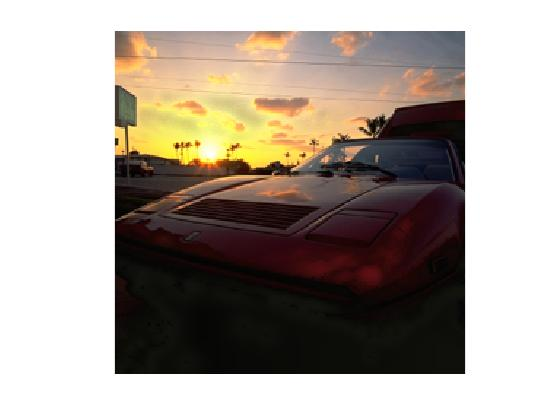
\includegraphics[width=1\textwidth]{images/ferrari_conc_tmr.jpg}
\caption{Le notre}
\end{minipage}
\end{figure}

\begin{figure}[h]
\centering
\begin{minipage}{0.33\textwidth}
\centering
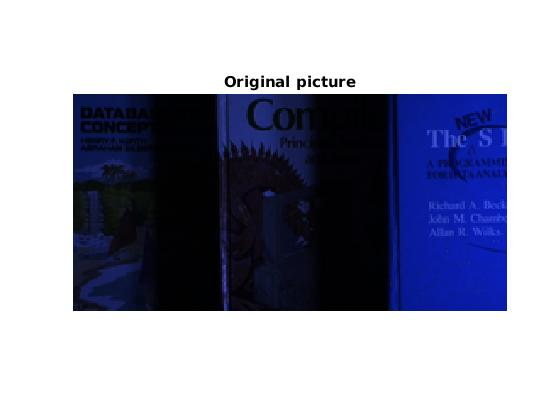
\includegraphics[width=1\textwidth]{images/book_conc_depart.jpg}
\caption{Original}
\end{minipage}%
\begin{minipage}{0.33\textwidth}
\centering
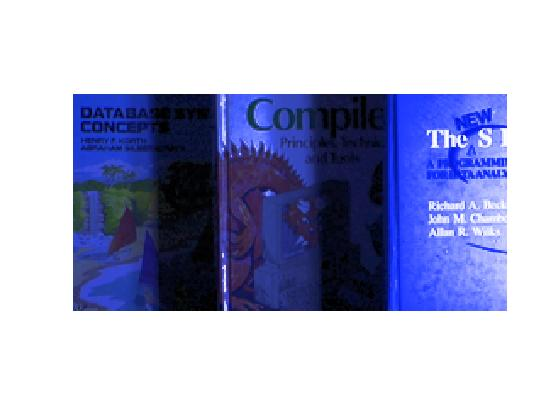
\includegraphics[width=1\textwidth]{images/book_conc_inter.jpg}
\caption{Naïf}
\end{minipage}%
\begin{minipage}{0.33\textwidth}
\centering
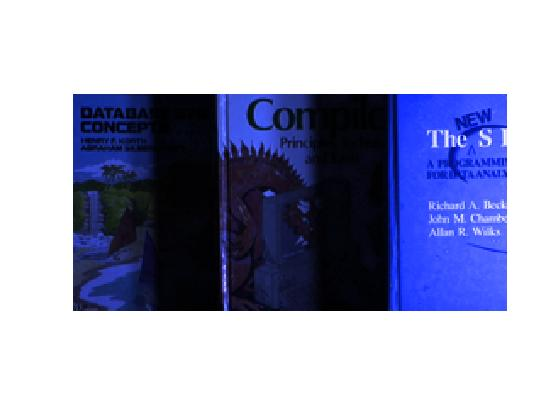
\includegraphics[width=1\textwidth]{images/book_conc_tmr.jpg}
\caption{Le notre}
\end{minipage}
\end{figure}

\begin{figure}[h]
\centering
\begin{minipage}{0.33\textwidth}
\centering
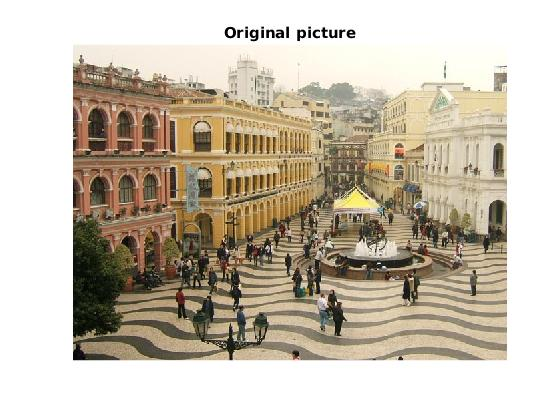
\includegraphics[width=1\textwidth]{images/macau_conc_depart.jpg}
\caption{Original}
\end{minipage}%
\begin{minipage}{0.33\textwidth}
\centering
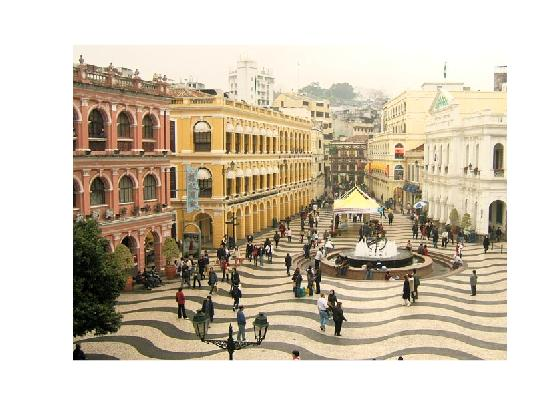
\includegraphics[width=1\textwidth]{images/macau_conc_inter.jpg}
\caption{Naïf}
\end{minipage}%
\begin{minipage}{0.33\textwidth}
\centering
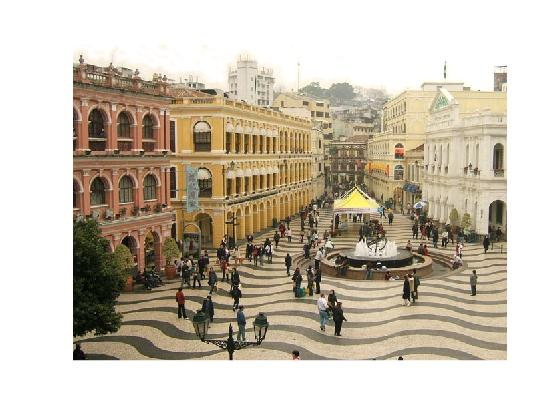
\includegraphics[width=1\textwidth]{images/macau_conc_tmr.jpg}
\caption{Le notre}
\end{minipage}
\end{figure}

\begin{figure}[h]
\centering
\begin{minipage}{0.33\textwidth}
\centering
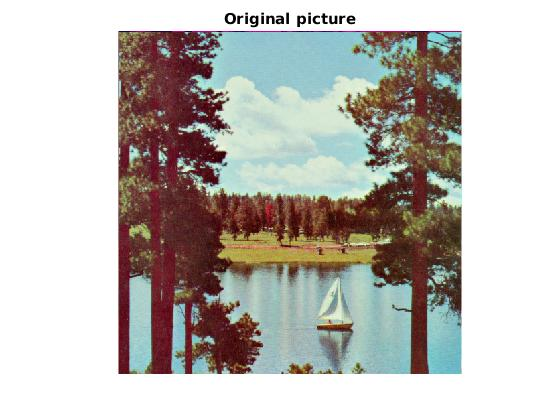
\includegraphics[width=1\textwidth]{images/sail_conc_depart.jpg}
\caption{Original}
\end{minipage}%
\begin{minipage}{0.33\textwidth}
\centering
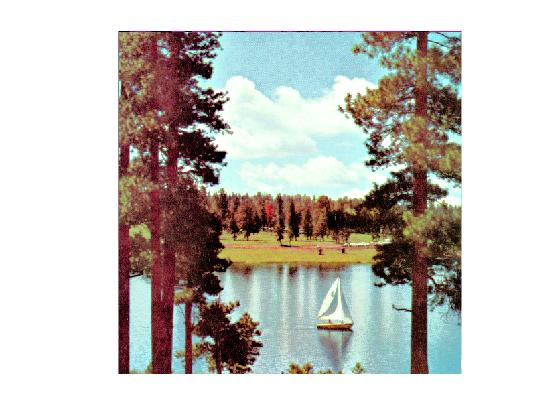
\includegraphics[width=1\textwidth]{images/sail_conc_inter.jpg}
\caption{Naïf}
\end{minipage}%
\begin{minipage}{0.33\textwidth}
\centering
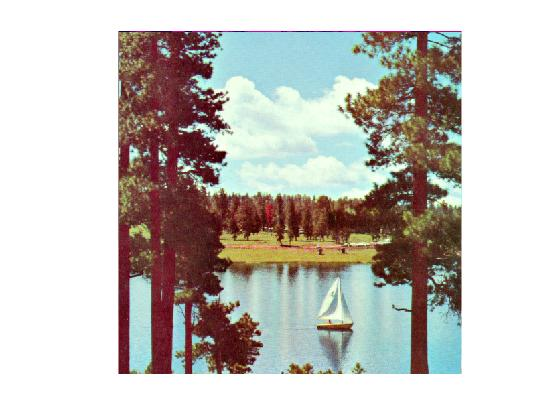
\includegraphics[width=1\textwidth]{images/sail_conc_tmr.jpg}
\caption{Le notre}
\end{minipage}
\end{figure}


\end{document}
